\chapter{Momentum}

Let's say a 2 kg block of putty is flying through space at 5 meters
per second, and it collides with a larger 3 kg block of putty that is not
moving at all. When the two blocks deform and stick to each other, how
fast will the resulting big block be moving?

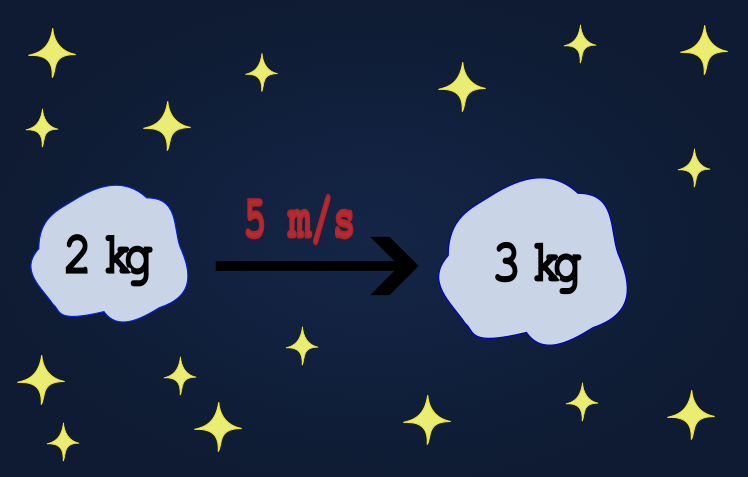
\includegraphics[width=0.4\textwidth]{Space_Putty.png}


Every object has \newterm{momentum}.  The momentum is a vector
quantity: It points in the direction that the object is moving and has
a magnitude equal to its mass times its speed.

Given a set of objects that are interacting, we can sum all their
momentum vectors to get the total momentum.  In such a set, the total
momentum will stay constant.

So, in our example, one object has a momentum vector of magnitude of
10 kg m/s, the other has a momentum of magnitude 0.  Once they have
merged, they have a combined mass of 5 kg.  Thus, the velocity vector
must have magnitude 2 m/s and pointing in the same direction that the
first mass was moving.

\begin{Exercise}[title={Cars on Ice}, label=cars_on_ice]
A car weighing 1000 kg is going north at 12 m/s.  Another car weighing
1500 kg is going east at 16 m/s.  They both hit a patch of ice (with
zero friction) and collide.  Steel is bent and the two objects become
one.  How what is the velocity vector (direction and magnitude) of the
new object sliding across the ice?
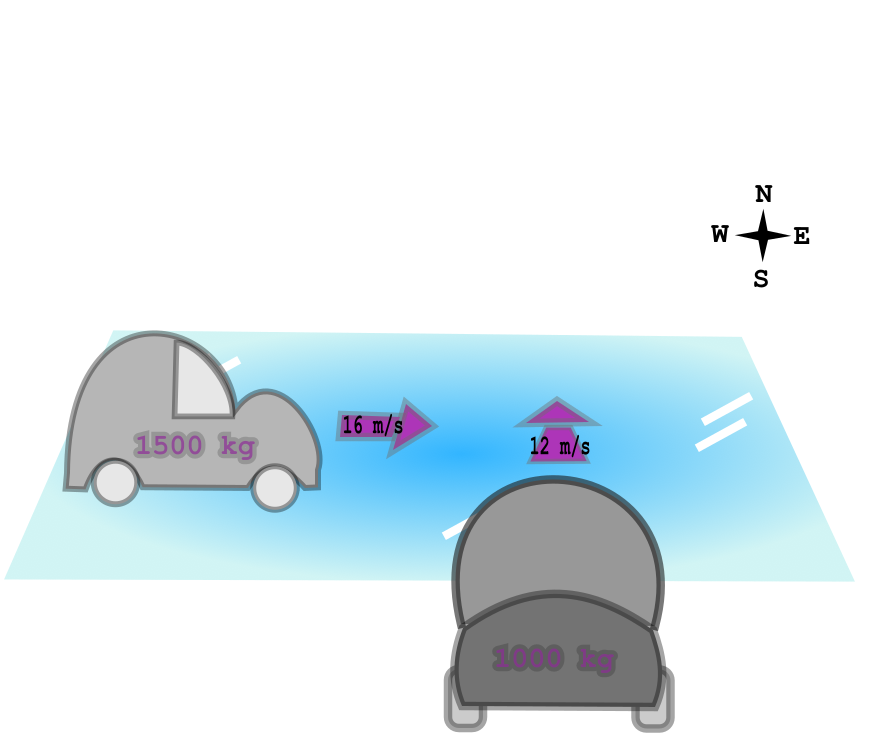
\includegraphics[width=0.4\textwidth]{Car_Ice.png}

\end{Exercise}
\begin{Answer}[ref=cars_on_ice]
  The momentum of the first car is 12,000 kg m/s in the north direction.

  The momentum of the second car is 24,000 kg m/s in the east direction.

  The new object will be moving northeast. What angle is the angle compared with the east?

  $$\theta = \arctan{\frac{12,000}{24,000}} \approx 0.4636 \text{ radians } \approx 26.565\text{ degrees north of east}$$

  The magnitude of the momentum of the new object is $\sqrt{12,000^2 + 24,000^2} \approx 26,833\text{ kg m/s}$

  Its new mass is 2,5000 kg.  So the speed will be $26,833/2,500 = 10.73$ m/s.
\end{Answer}


Notice that kinetic energy ($1/2 m v^2$) is \emph{not} conserved
here.  Before the collision, the moving putty block has $(1/2)(2)(5^2) = 25$
joules of kinetic energy.  Afterward, the big block has $(1/2)(5)(2^2)
= 10$ joules of kinetic energy.  What happened to the energy that was
lost? It was used up deforming the putty.

What if the blocks were marble instead of putty?  Then there would be
very little deforming, so kinetic energy \emph{and} momentum would be
conserved. The two blocks would end up having different velocity
vectors.

Let's assume for a moment that they strike each other straight on, so
there is motion in only one direction, both before and after the
collision.  Can we solve for the speeds of the first block ($v_1$) and
the second block ($v_2$)?

We end up with two equations. Conservation of momentum says:

$$2 v_1 + 3 v_2 = 10$$

Conservation of kinetic energy says:

$$(1/2)(2)(v_1^2) + (1/2)(3)(v_2^2) = 25$$

Using the first equation, we can solve for $v_1$ in terms of $v_2$:

$$v_1 = \frac{10 - 3 v_2}{2}$$

Substituting this into the second equation, we get:

$$\left(\frac{10 - 3 v_2}{2}\right)^2 + \frac{3 v_2^2}{2} = 25$$

Simplifying, we get:

$$v_2^2 - 4 v_2 + 0 = 0$$

This quadratic has two solutions: $v_2 = 0$ and $v_2 = 4$.  $v_2 = 0$
represents the situation before the collision.  Substituting in $v_2 = 4$:

$$v_1 = \frac{10 - 3(4)}{2} = -1$$

Thus, if the blocks are hard enough that kinetic energy is conserved,
after the collision, the smaller block will be heading in the opposite
direction at 1 m/s.  The larger block will be moving at 4 m/s in the
direction of the original motion.

\begin{Exercise}[title={Billiard Balls}, label=billiards]
  
A billiard ball weighing 0.4 kg and traveling at 3 m/s hits a billiard
ball (same weight) at rest. It strikes obliquely so that the ball at rest starts to
move at a 45 degree angle from the path of the ball that hit it.

Assuming all kinetic energy is conserved. How what is the velocity
vector of each ball after the collision?

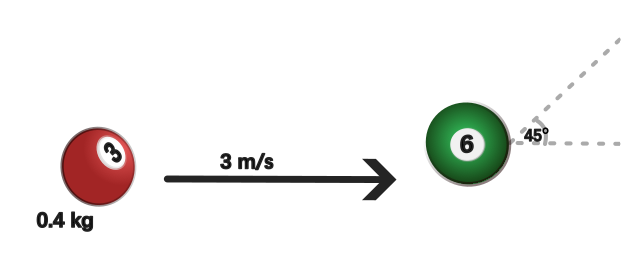
\includegraphics[width=0.4\textwidth]{billiards.png}

\end{Exercise}
\begin{Answer}[ref=billiards]

  The original forward momentum was 1.2 kg m/s.  The original kinetic energy is $(1/2)(0.4)(3^2)$ = 1.8 joules. 

  Let $s$ be the post-collision speed of the ball that had been at
  rest.  Let $x$ and $y$ be the forward and sideways speeds
  (post-collision) of the other ball. Conservation of kinetic energy says

  $$(1/2)(0.4)(s^2) + (1/2)(0.4)(x^2+y^2) = 1.8$$

  Forward momentum is conserved:

  $$0.4\frac{s}{\sqrt{2}} + 0.4 x = 1.2$$

  Which can be rewritten:

  $$x = 3 - \frac{s}{\sqrt{2}}$$
  
  Sideways momentum stays zero:

  $$(0.4)\frac{s}{\sqrt{2}} - 0.4 y = 0.0$$

  Which can be rewritten:

  $$y = \frac{s}{\sqrt{2}}$$

  Substituting into to the conservation of kinetic energy equation above:

  $$(1/2)(0.4)(s^2) + (1/2)(0.4)(\left(3 - \frac{s}{\sqrt{2}}\right)^2+\left(\frac{s}{\sqrt{2}}\right)^2 = 1.8$$

  Which can be rewritten:

  $$s^2 - \frac{3}{\sqrt{2}} s + 0 = 0$$

  There are two solutions to this quadratic: $s = 0$ (before collision) and $s = \frac{3}{\sqrt{2}}$. Thus,

  $$y = \frac{3}{2}$$

  and

  $$x = 3 - \frac{3}{2} = \frac{3}{2}$$

  So both balls careen off at $45^\circ$ angles at the exact same speed. 

  
\end{Answer}



